\documentclass[a4paper,12pt]{article}
\usepackage{graphicx}
\usepackage[left=30mm, right=30mm, top=30mm, bottom=30mm]{geometry}
\usepackage{amsmath}
\usepackage{siunitx}
\usepackage{fancyhdr}
\usepackage{url}
\pagestyle{fancy}
%-------------------------------------------------------------------------------
\lhead{\textbf{CE394M}}
\rhead{\textbf{Advanced Analysis in Geotechnical Engineering}}
\cfoot{\thepage}
%-------------------------------------------------------------------------------

\begin{document}
\begin{centering}
	\textbf{
		Assignment 8: Elastic-Perfectly Plastic Finite Element Analysis\\
	}
\end{centering}

\vspace{1em}
 
\begin{enumerate}

	\item  Using the Soil Test option within the finite element program PLAXIS 2D, analyze the
	response of an isotropically consolidated triaxial specimen under drained loading in triaxial
	compression. Assume that the soil can be modeled as a linear elastic-perfectly plastic
	material (Mohr-Coulomb model in PLAXIS). Please read Section 3 of the Material Models
	Manual for background on this soil model.
	
	Again, consider the consolidated-drained triaxial test data for a sand found in hw3-tx-data.xlsx posted on Canvas. Use the triaxial data to determine $\phi^\prime$ (assume $c^\prime = 0 kPa$), and use this value along with the baseline linear elastic parameters from Homework 7 ($E^\prime = E_{0.5\%}, \nu^\prime = 0.2, \gamma_t = 18 kN/m^3, and \psi^\prime = 0^o$) to define the Mohr-Coulomb parameters for this sand.
	Isotropically load the triaxial specimen in PLAXIS to a confining stress of 100 kPa, and
	compute the response up to an axial strain of 5\%.
	
	\begin{enumerate}
		\item For this baseline case, plot the results in the familiar deviator stress ($q = \sigma_1 - \sigma_3$) vs. axial
		strain and volumetric strain vs. axial strain. Check the predicted yield stress and
		associated volumetric strain from PLAXIS with a hand calculation. Compare the
		predicted curves with those from the triaxial test and discuss any differences.
		
		\item Vary $\phi^\prime \pm 5^o$, plot the results, and comment on the influence of $\phi^\prime$ on the results

		\item Analyze the baseline conditions with $\psi^\prime + 3^o$ and $+10^o$. For the  $\psi^\prime = 3^o$, confirm the
		predicted volumetric strain at an axial strain of 5\% with a hand calculation. Plot the
		results and comment on the influence of $\phi^\prime$ on the results.
		
		\item Repeat the baseline analysis for an undrained loading. Plot deviator stress vs. axial strain, volumetric strain vs. axial strain, and pore water pressures vs. axial strain. Comment on the undrained vs. drained response of the soil.
		\item Repeat the undrained analysis with $\psi^\prime = 10^o$. Plot deviator stress vs. axial strain,
		volumetric strain vs. axial strain, and pore water pressures vs. axial strain. Comment
		on the influence of $phi^\prime$ the undrained response.
	\end{enumerate}
	
	\item Using the finite element program PLAXIS with the Mohr-Coulomb model, analyze the plane
	strain problem of a long strip surface loading of a finite, elastic-perfectly plastic soil layer
	underlain by a rigid base (see figure below). There is no water; hence, effective stresses
	equal total stresses. For the baseline case, use: $E^\prime = 20,000 kPa, \nu^\prime = 0.2, c^\prime = 5 kPa, \phi^\prime = 36^o, \phi^\prime = 0^o, \gamma_t = 18 kN/m^3, K_0 = 0.6, H = 10m, q = 250 kPa$, and $B = 3 m$.  The soil is treated as an
	existing foundation with no water, and the surface load as an applied distributed load. Use a
	``medium'' mesh of 15-node triangles in this analysis. Examine the results from the FE
	analysis to observe the distribution of displacements, strains, and stresses across the region.	Specifically:
	
	\begin{enumerate}
		\item Show a plot of the finite element mesh used in your baseline analysis with the deformed mesh for the baseline case. Show the
		distribution of shear stress level ($\tau_{rel}$ in PLAXIS) within the finite element domain.
		\item Compare the results (i.e., vertical and horizontal displacements at the edge of the
		strip loading and the vertical stress versus depth beneath the edge of the strip
		loading) for the Mohr-Coulomb case and the linear elastic case from the linear elastic Homework 7.
		\item Evaluate the sensitivity of the results (i.e., displacements at the edge of the
		loading, distribution of shear stress level) to the finite element model employed in
		the analysis by re-analyzing the baseline case using a ``very coarse'' mesh of 6-
		node triangles.
		\item Evaluate the sensitivity of the results (i.e., displacements at the edge of the
		loading, distribution of shear stress level) to variations in the input parameters
		$K_o, \phi^\prime, and \psi^\prime$. Specifically, perform analyses where the following changes to the
		baseline parameters are made: (1) $K_0 = 0.4$, (2) $\phi^\prime = 33^o$, (3) $\phi^\prime = 39^o$, (4) $\psi^\prime = 3^o$ and (5) $\psi^\prime = 10^o$
	\end{enumerate}

	\begin{figure}[!h]
		\centering
		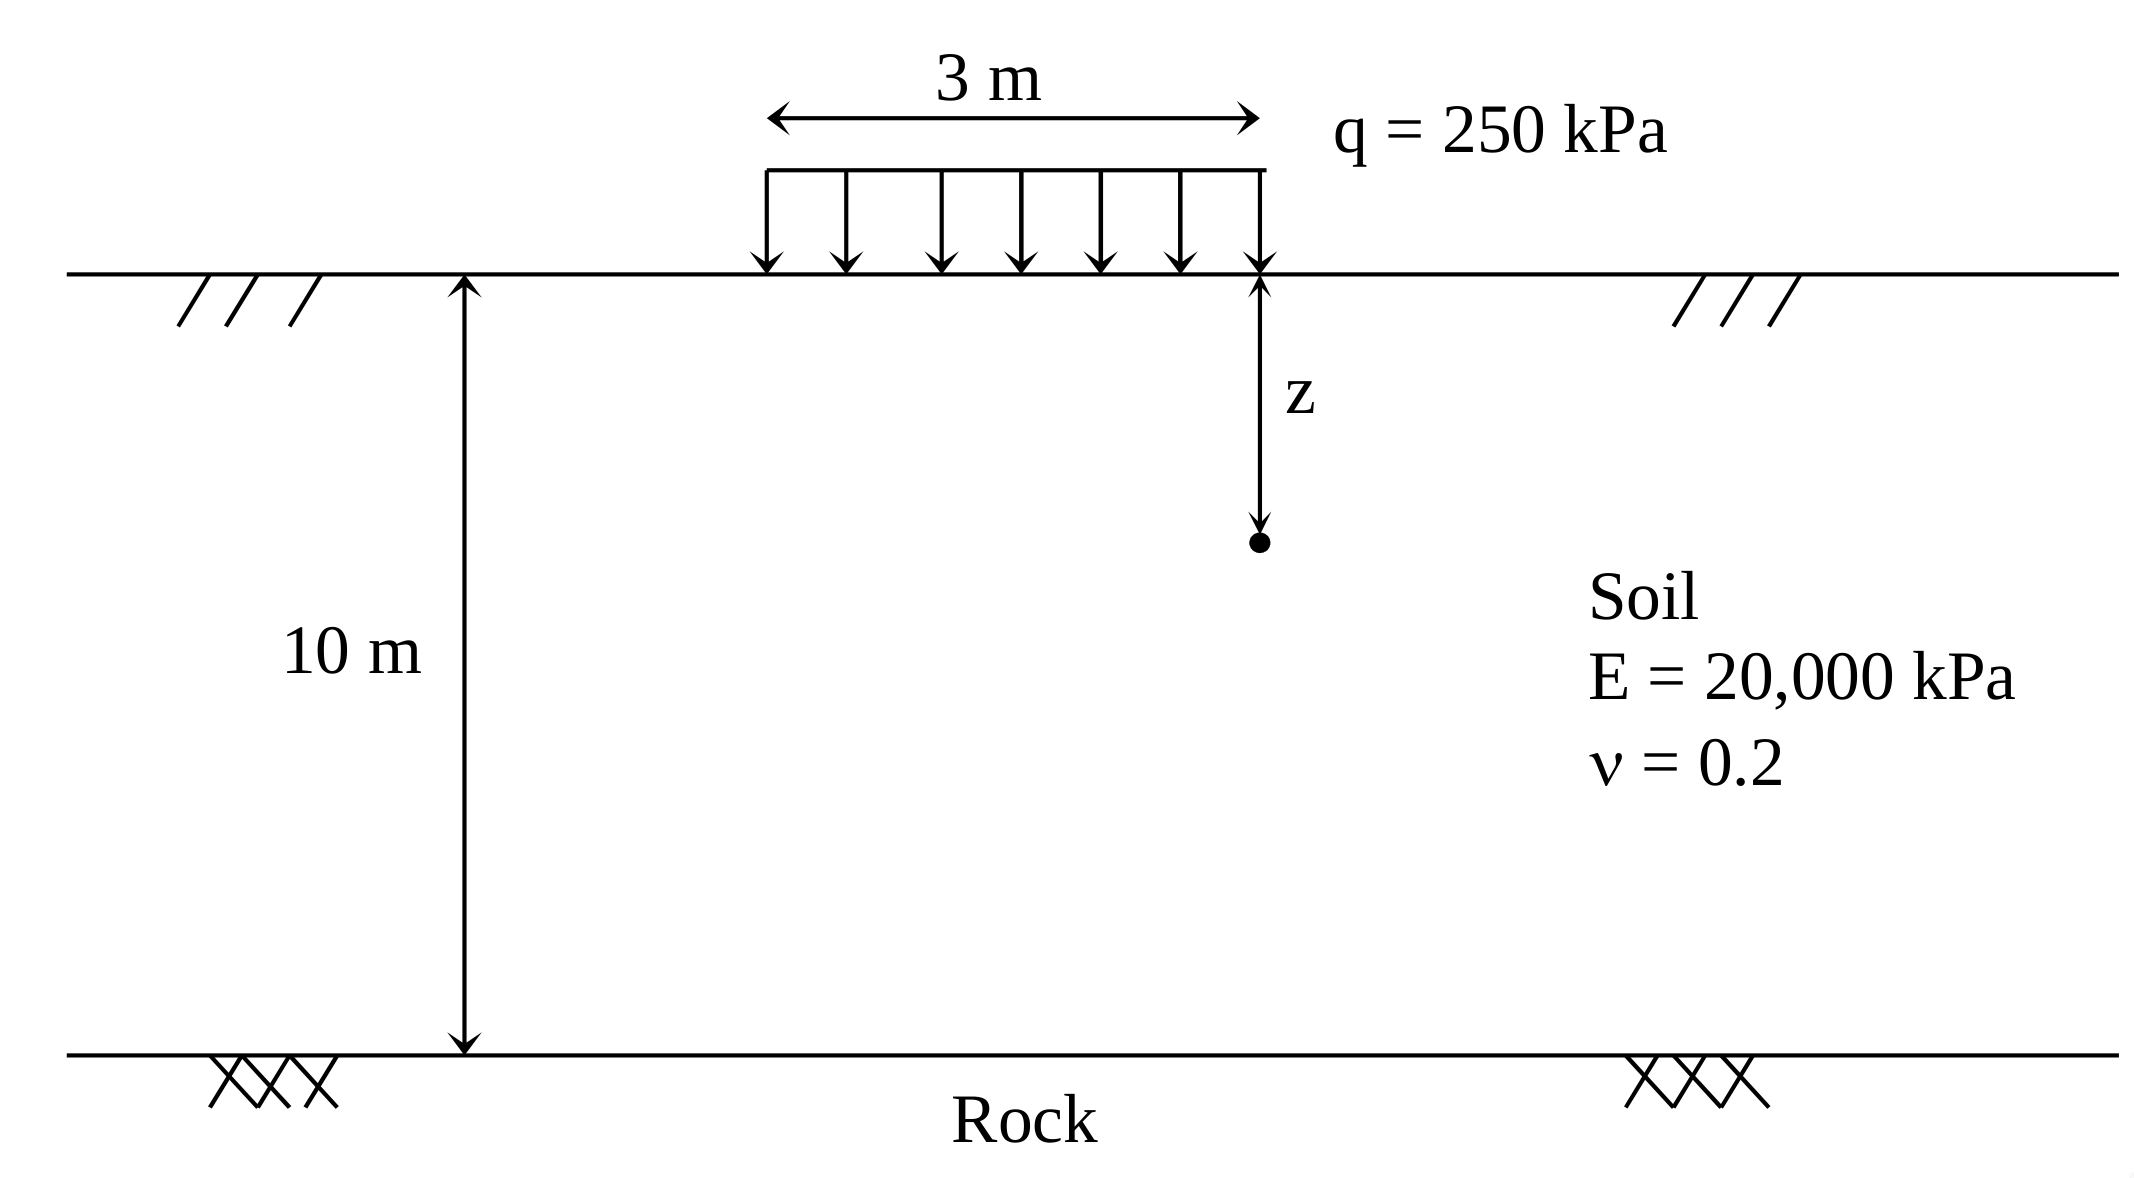
\includegraphics[width=0.85\textwidth]{figs/footing.png}
	\end{figure}
\end{enumerate}

\end{document}

